\documentclass{article}

\usepackage[margin=1in]{geometry}
\usepackage{amsmath,amsthm,amssymb}
\usepackage{bbm,enumerate,mathtools}
\usepackage{tikz}

\newenvironment{question}{\begin{trivlist}\item[\textbf{Question.}]}{\end{trivlist}}
\newenvironment{note}{\begin{trivlist}\item[\textbf{Note.}]}{\end{trivlist}}
\newenvironment{references}{\begin{trivlist}\item[\textbf{References.}]}{\end{trivlist}}
\newenvironment{related}{\begin{trivlist}\item[\textbf{Related.}]\end{trivlist}\begin{enumerate}}{\end{enumerate}}
\begin{document}

\title{Problem 6.}
\date{}
\author{Peter Kagey}
\maketitle

  Let \[
    C_n = \{f: [n] \rightarrow \mathbb{N}\ |\ \text{the convex hull around } \{(1, f(1)), \hdots, (n, f(n))\} \text{ forms an } n\text{-gon}\}
  \] and then let $a(n)$ denote the least upper bound over all functions in $C_n$ \[
    a(n) = \min\{\max\{f(k)\ |\ k \in [n]\}\ |\ f \in C_n\}
  \]
\begin{figure}[!h]
  \centering
  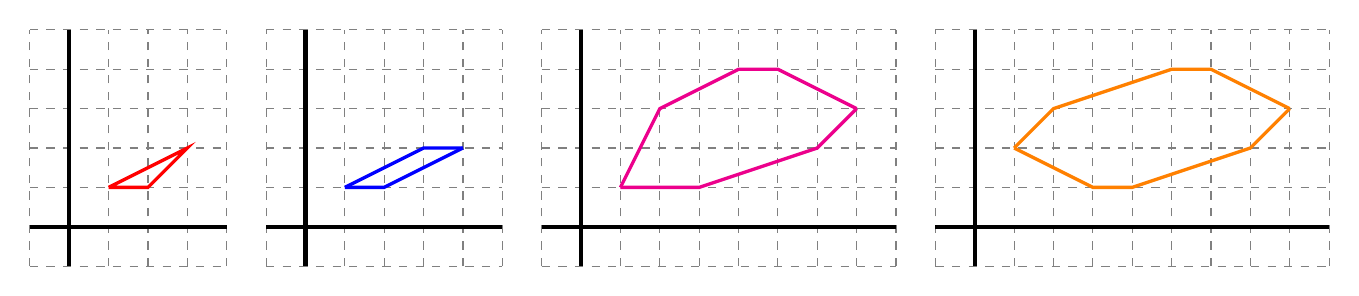
\begin{tikzpicture}[scale=0.5]
    \draw[gray, dashed] (-1,-1) grid (4,5);
    \draw[ultra thick,black] (-1,0) -- (4,0);
    \draw[ultra thick,black] (0,-1) -- (0,5);
    \draw[red,very thick] (1,1) -- (2,1) -- (3,2) -- (1,1);

% --------------------------------------------
    \draw[gray,dashed] (5,-1) grid (11,5);
    \draw[ultra thick,black] (5,0) -- (11,0);
    \draw[ultra thick,black] (6,-1) -- (6,5);

    \draw[blue,very thick] (7,1) -- (8,1) -- (10,2);
    \draw[blue,very thick] (7,1) -- (9,2) -- (10,2);

    % --------------------------------------------
    \draw[gray,dashed] (12,-1) grid (21,5);
    \draw[ultra thick,black] (12,0) -- (21,0);
    \draw[ultra thick,black] (13,-1) -- (13,5);
    \draw[magenta,very thick] (14,1) -- (16,1) -- (19,2) -- (20,3);
    \draw[magenta,very thick] (14,1) -- (15,3) -- (17,4) -- (18,4) -- (20,3);

    \draw[gray,dashed] (22,-1) grid (32,5);
    \draw[ultra thick,black] (22,0) -- (32,0);
    \draw[ultra thick,black] (23,-1) -- (23,5);

    \draw[orange,very thick] (24,2) -- (25,3) -- (28,4) -- (29,4) -- (31,3);
    \draw[orange,very thick] (24,2) -- (26,1) -- (27,1) -- (30,2) -- (31,3);
  \end{tikzpicture}
  \caption{Examples of $a(3) = 2$, $a(4) = 2$, $a(7) = 4$, and $a(8) = 4$, where
    the polygons with an even number of vertices have rotational symmetry.}
\end{figure}

\begin{question}
  Do these polygons converge to something asymptotically?
\end{question}

\begin{related}
  \item Does $a(2n) = a(2n - 1)$ for all $n$?
  \item Do the minimal $2n$-gons always have a representative with rotational
    symmetry?
  \item Are minimal $2n$-gons unique (up to vertical symmetry) with finitely
    many counterexamples?
  \item What is the asymptotic growth of a(n)?
\end{related}

\begin{references} \text{} \\
  A285521: ``Table read by rows: the n-th row gives the lexicographically earliest sequence of length n such that the convex hull of (1, a(1)), ..., (n, a(n)) is an n-gon with minimum height.'' (https://oeis.org/A285521)
\end{references}

\end{document}
